%\documentclass{beamer}
%\documentclass[handout]{beamer}
%\documentclass[12pt,handout]{beamer}
\documentclass[12pt,donthandout,notes=dontshow,xcolor=table]{beamer}

\NeedsTeXFormat{LaTeX2e}
\usepackage[orientation=landscape,size=custom,width=16,height=9,scale=.5,debug]{beamerposter} 
\usepackage[utf8]{inputenc}
\usepackage[german]{babel}      % Sprachanpassungen für generierte Texte wie "Inhaltsverzeichnis" etc

%\usepackage[table]{xcolor}
\usepackage{tabularx}
\usepackage{textcomp}
\usepackage{tikz}
\usetikzlibrary{shapes,arrows,positioning,trees,shadings,decorations.pathreplacing,backgrounds}
\usepackage{tcolorbox}
\usepackage{pdfpages}
\usepackage{listings}
\usepackage{longtable}

\usepackage{minted}

%\usetheme{Madrid}
\usetheme{Goettingen}


%\usepackage{etoolbox}  % http://dante.ctan.org/tex-archive/help/Catalogue/entries/etoolbox.html
\usepackage[
        hyperref=true,          % Klickbare Referenzen in der PDF-Datei
        %backref=true,           % In der Literaturref. die Seiten angeben, wo ein \cite dazu steht
        bibencoding=inputenc,   % s. inputenc-Paket
        style=numeric,
        backend=bibtex,
        sorting=nty]{biblatex}  % http://dante.ctan.org/tex-archive/help/Catalogue/entries/biblatex.html
\renewcommand{\mkbibnamelast}[1]{\textsc{#1}}
\bibliography{presentation}

%%%%%%%%%%% PRINT NOTES
%\usepackage{pgfpages}
%\pgfpagesuselayout{2 on 1}[a4paper]
%\setbeameroption{show notes on second screen=bottom} % Beamer manual, section 19.3
%\usetemplatenote{\beamertemplatefootempty \insertnote}
%%%%%%%%%%% PRINT NOTES

%\useoutertheme{shadow}
%\setbeamertemplate{items}[default]
\beamertemplatenavigationsymbolsempty
\setbeamertemplate{footline}[frame number]

\author{Sebastian Bernauer}
\title{NP-Vollständigkeit wichtiger Probleme}

%\AtBeginSection[]
%{
%	\begin{frame}{Inhalt}
%	\tableofcontents[currentsection]
%	\end{frame}
%}

\begin{document}

\begin{frame}
\titlepage
\end{frame}

\begin{frame}[allowframebreaks]
\frametitle{Inhalt}
\tableofcontents
\end{frame}

%\section{3-SAT}
%\subsection{Problem}
%\begin{frame}{3-SAT Problem}
%Problem
%\end{frame}
%
%\subsection{Beweis}
%\begin{frame}{3-SAT Beweis}
%Beweis
%\end{frame}

\section{Komplexitätsklassen}
\begin{frame}{Komplexitätsklassen}
\textbf{Definition:} \(\leq_p\) ``ordnet'' Entscheidungsprobleme bezüglich ihrer Komplexität.\\
Aufsteigende Komplexitätsklassen:
\begin{enumerate}
\item P - polynomiell lösbar
\pause
\item NP - nichtdeterministisch polynomiell lösbar
\pause
\item NP-schwierig\\
\textrightarrow \(\forall L` \in NP: L` \leq_p L\)
\pause
\item NP-vollständig\\
\textrightarrow \(L \in NP\) und \(\forall L` \in NP: L` \leq_p L\)\\
\pause
\textrightarrow Alle folgenden Probleme sind NP-vollständig
\pause
\item nicht rekursiv
\end{enumerate}
\end{frame}

\section{Satisfiability Problem (SAT)}
\begin{frame}{Satisfiability Problem}
Für natürliche Zahlen \(n\) und \(m\) seien \(m\) Klauseln über \(n\) Variablen gegeben.
Eine Klausel ist die Disjunktion [Veroderung] von einigen Literalen \(x_i\) bzw. \(\overline{x_i}\) mit \(i,j \in \{1,...,n\}\). Es soll entschieden werden, ob es eine Belegung \(a = \{a_1,...,a_n\} \in \{0,1\}^n\) der Variablen \(x_1,...,x_n\) gibt, so dass alle Klauseln erfüllt sind.\\
\pause
\textbf{Fragestellung:} Existiert eine Wahrheitsbelegung der Variablen \(x_1,...,x_n\), so dass alle Klauseln erfüllt sind?\\
\pause
\textrightarrow Satz von Cook: SAT is NP-vollständig
\end{frame}

\subsection{3-SAT}
\begin{frame}{3-SAT}
\begin{itemize}
\item Spezialfall von SAT
\item Jede Klausel enthält 3 Literale
\item Zu Beweisen: SAT ist durch 3-SAT abbildbar und beide sind damit gleich komplex (NP-vollständig)
\end{itemize}
\end{frame}

\subsection{Beweis: 3-SAT $\leq_p$ SAT}
\begin{frame}{Beweis: 3-SAT \(\leq_p\) SAT}
\begin{itemize}
\item Klausel 1 Literal  \(z\) \\ \textrightarrow \(z \vee z \vee z\)
\item Klausel 2 Literale \(z \vee y\) \\ \textrightarrow \(z \vee z \vee y\)
\item Klausel 3 Literale \(z \vee y \vee z\) \\ \textrightarrow Keine Änderung
\item Klausel \(\ge\) 4 Literale \(z_1 \vee ... \vee z_k\) \\ \textrightarrow siehe nächste Folie
\end{itemize}
\end{frame}

\begin{frame}{Beweis: 3-SAT \(\leq_p\) SAT}
Beispiel: \(k = 7\) mit \(z_1 \vee ... \vee z_k\):
\begin{itemize}
\item \(z_1 \vee z_2 \vee y_1\)
\item \(\overline{y_1} \vee z_3 \vee y_2\)
\item \(\overline{y_2} \vee z_4 \vee y_3\)
\item \(\overline{y_3} \vee z_5 \vee y_4\)
\item \(\overline{y_4} \vee z_6 \vee z_7\)\\
\end{itemize}
\end{frame}

\begin{frame}{Beweis: 3-SAT \(\leq_p\) SAT}
\begin{itemize}
\item SAT lässt sich durch 3-SAT abbilden
\item 3-SAT \(\leq_p\) SAT
\item 3-SAT ist NP-vollständig
\end{itemize}
\end{frame}

\section{Clique Problem}
\begin{frame}{Clique Problem}
In einem ungerichteten Graphen $G = (V,E)$ bildet die Knotenmenge $V` \subseteq V$ eine Clique, wenn für alle $v, v` \in V`$ gilt ${v,v`} \in E$. \cite{wegener}
\pause
\begin{figure}
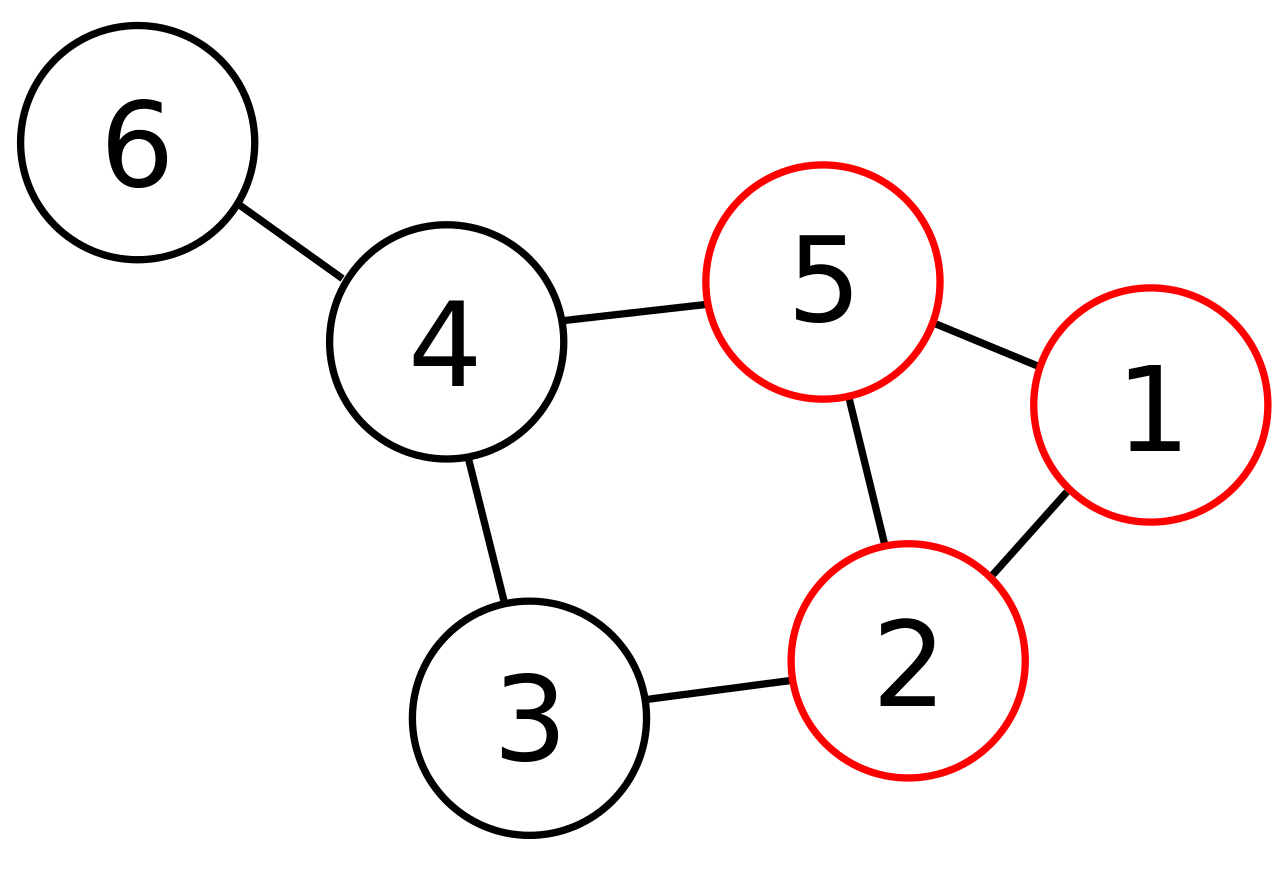
\includegraphics[width=6cm]{figures/clique1.png}
\caption{Ein Graph mit einer Clique der Größe 3.\newline \newline \tiny Quelle: https://de.wikipedia.org/wiki/Clique\_(Graphentheorie)\#/media/File:6n-graf-clique.svg}
\end{figure}
\end{frame}

\begin{frame}{Clique - Beispiel}
\begin{figure}
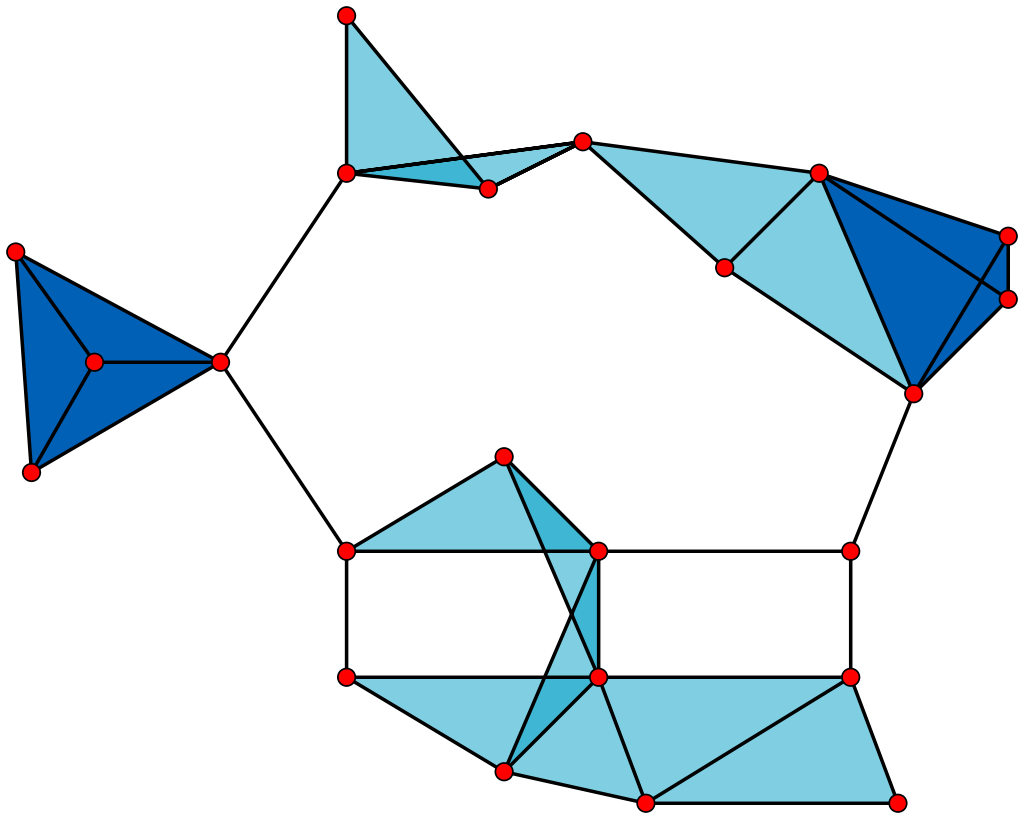
\includegraphics[width=6cm]{figures/clique2.png}
\caption{Ein Graph mit 2 Cliquen der Größe 4.\newline \newline \tiny Quelle: https://en.wikipedia.org/wiki/Clique\_(graph\_theory)\#/media/File:VR\_complex.svg}
\end{figure}
\end{frame}

\begin{frame}{Clique - Fragestellungen}
\begin{enumerate}
\item Gibt es eine Clique der Größe k?\\
\textrightarrow Entscheidungsproblem
\newline \pause
\item Berechne das größte k, so dass eine Clique der Größe k vorhanden ist.\\
\textrightarrow Optimale Lösung
\newline \pause
\item Berechne eine Clique mit dem größten k.\\
\textrightarrow Optimierungsproblem
\end{enumerate}
\end{frame}

\subsection{Beweis}
\begin{frame}{Clique - Beweis}
Clique ist in NP enthalten.\\
Beweis:\\
\begin{enumerate}
\item NTM zählt Anzahl \(n\) der Knoten im Graphen
\pause
\item Rät Wort \(w \in \{0,1\}^n\)
\pause
\item Das Wort wird als Knotenauswahl interpretiert, \(V'\) enthält alle Knoten \(i\) mit \(w_i = 1\)
\pause
\item Es wird getestet, ob
\begin{enumerate}
\item \(V'\) genau \(k\) Knoten beinhaltet.
\item \(G\) eine Clique auf \(V'\) enthält
\end{enumerate}
\end{enumerate}
\pause
\begin{itemize}
\item Rechenaufwand ist polynomiell in der Knotenzahl \(n\)
\end{itemize}
\end{frame}

\begin{frame}{Clique - Beweis}
\begin{itemize}
\item NTM können durch DTM abgebildet werden
\item Polynomielle Laufzeit + Nichtdeterminismus => NP
\item Clique ist in NP enthalten
\end{itemize}
\end{frame}

\begin{frame}{Clique - Beweis}
Es wurde bereits bewiesen, dass \(Clique \in NP\) und \(SAT\) (und \(3-SAT\)) NP-vollständig ist.\\
Nun ist zu beweisen, dass \(SAT \leq_p Clique\).\\
Daraus folgt: \(Clique\) ist NP-vollständig.
\end{frame}

\begin{frame}{Clique - Beweis}
Konstruiere einen Graphen, der mittels \(Clique\) ein Problem löst, welches ein \(SAT\)-Problem ist.
\begin{enumerate}
\item Füge für jedes Literal in den Klauseln einen Knoten hinzu.
\pause
\item Verbinde alle Literale außer folgende Kanten:
\begin{itemize}
\item Klauselgruppen untereinander
\item Gegensätzliche Literale (z.B. \(x_1\) und \(\overline{x_1}\))
\end{itemize}
\pause
\item Suche eine Clique der Größe k, k ist die Anzahl der Klauseln. Da die Knoten einer Klauselgruppe nicht verbunden sind, muss aus jeder Klausel ein Literal ``wahr'' sein. Da die Literale in den Klauseln ODER-verknüpft sind, sind alle Klauseln erfüllt.\\
\end{enumerate}
\end{frame}

\begin{frame}{Clique - Beweis}
\begin{figure}
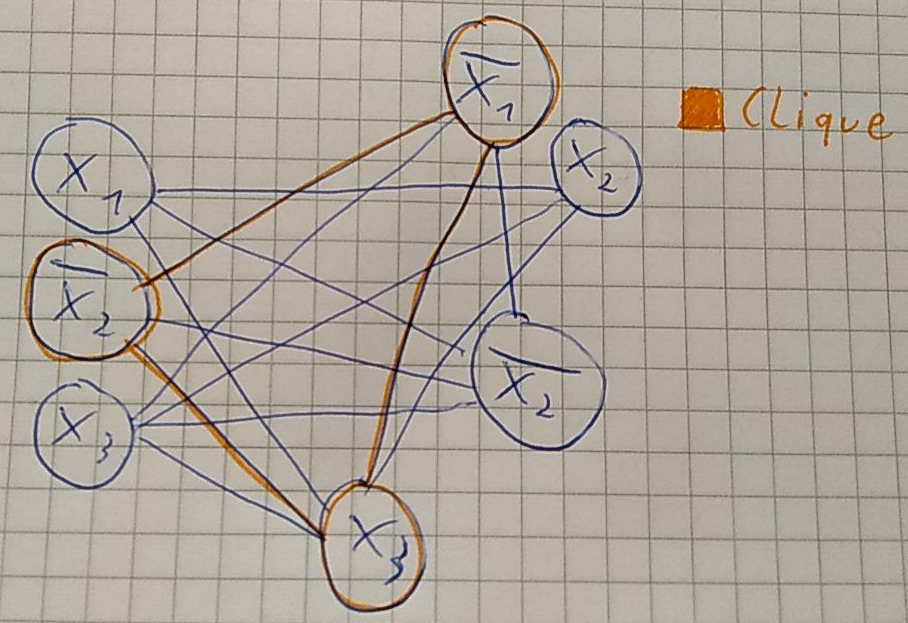
\includegraphics[width=9cm]{figures/clique_sat}
\caption{Graph nach Transformation von Clique- in SAT-Problem}
\end{figure}
\end{frame}

\begin{frame}{Clique - Beweis}
\textrightarrow \(SAT\)-Probleme können in ein \(Clique\)-Problem transferiert werden (mit polynomialen Zeitaufwand).\\
\textrightarrow \(Clique\) ist NP-vollständig.
\end{frame}

\section{Knapsack Problem}
\begin{frame}{Knapsack Problem}
Gegeben sind ein Rucksack und \(n\) Objekte mit Gewichten \(g_1,...,g_n \in \mathbb{N}\) sowie eine Gewichtsschranke \(G\).
Zusätzlich seien \(a_1,...,a_n \in \mathbb{N}\) die Nutzenwerte für die Objekte. \cite{wegener}
\pause
\begin{figure}
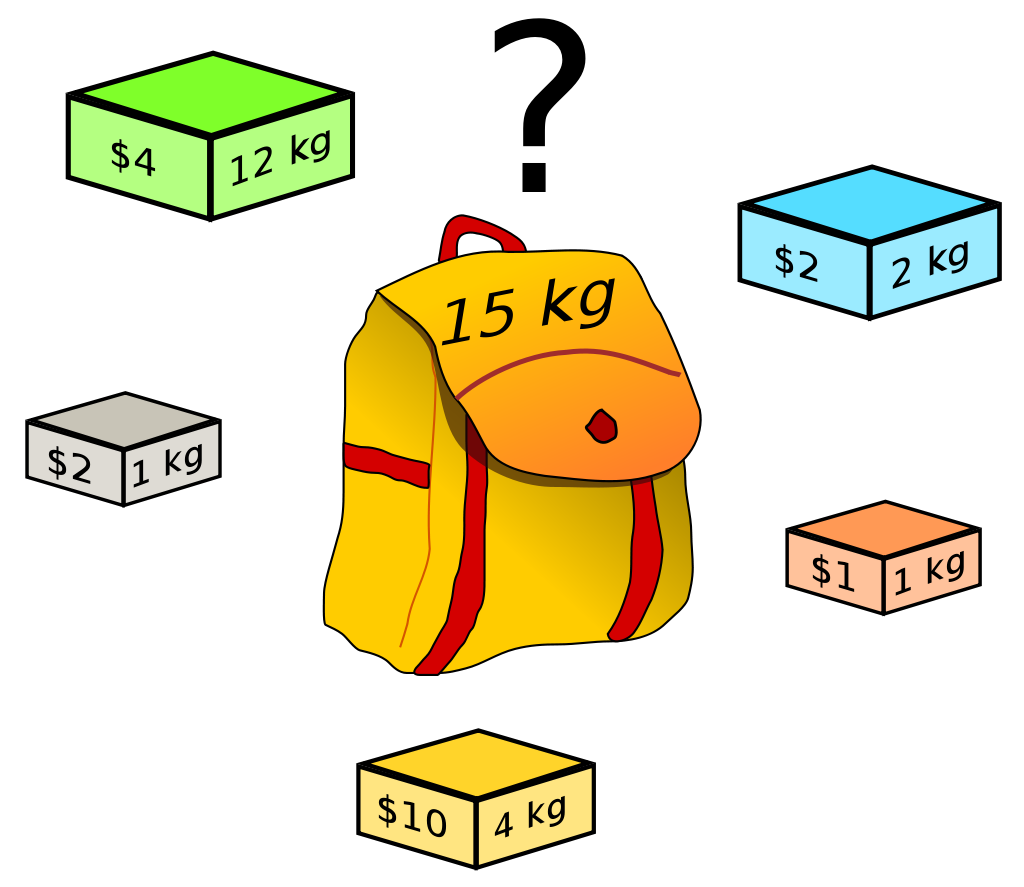
\includegraphics[width=4cm]{figures/knapsack.png}
\caption{Ein zu befüllender Rucksack.\newline \newline \tiny Quelle: https://de.wikipedia.org/wiki/Rucksackproblem\#/media/File:Knapsack.svg}
\end{figure}
\end{frame}

\begin{frame}{Knapsack - Fragestellungen}
\begin{enumerate}
\item Gibt es - unter Beachtung des Limits - eine Beladung mit mindestens diesem Nutzwert?\\
\textrightarrow Entscheidungsproblem
\newline \pause
\item Berechne den größtmöglichen Nutzwert.\\
\textrightarrow Optimale Lösung
\newline \pause
\item Berechne die optimale Beladung.\\
\textrightarrow Optimierungsproblem
\end{enumerate}
\end{frame}

\subsection{Beweis}
\begin{frame}{Knapsack - Beweis}
Beweis
\end{frame}



\section{Partition Problem}
\begin{frame}{Partition Problem}
Gegeben sind \(b_1,...,b_n \in \mathbb{N}\). Gibt es eine Teilmenge \(I \subseteq \{1,...,n\}\), so dass die Summe aller \(b_i, i \in I\) gleich der Summe aller \(b_i, i \notin I\) ist?\\
\textrightarrow Teil eine Menge von Gewichten in 2 gleich schwere Haufen auf.
\end{frame}

\subsection{Beweis}
\begin{frame}{Partition - Beweis}
Es wurde bereits bewiesen, dass ein spezielles Knapsack Problem \(KP\mbox{*}\) NP-vollständig ist.\\
(Für \(a_1,...,a_n\) soll entschieden werden, ob es eine Auswahl gibt, so dass die Summe genau \(A\) beträgt).\\
Nun ist zu beweisen, dass \(KP\mbox{*} \leq_p PARTITION\).\\
Daraus folgt: \(PARTITION\) ist NP-vollständig.
\end{frame}

\begin{frame}{Partition - Beweis}
Sei \((a_1,...,a_n,A)\) eine Eingabe für \(KP\mbox{*}\).\\
Daraus konstruieren wir in polynomieller Zeit die Eingabe\\
\((a_1,...,a_n,S-A+1,A+1)\) für \(PARTITION\), wobei \(S\) die Summe aller \(a_i\) ist.\\
Falls \(I\) eine Lösung für das \(KP\) ist, erhalten wir mit \(I \cup \{n+1\}\) eine Lösung für \(PARTITION\), da\\
$$\sum_{i \in I}a_i + S - A + 1 = S + 1 = \sum_{1 \le i \le n}a_i + 1 = \sum_{i \notin I}a_i + A + 1$$\\
Sie Summe aller Zahlen in der Eingabe für \(PARTITION\) beträgt \(2S + 2\).
Ein Lösung für \(PARTITION\) muss also so aussehen, dass jeder Teil sich zu \(S + 1\) aufsummiert.
Damit müssen die Zahlen \(S - A + 1\) und \(A + 1\) in verschiedenen Teilen sein.
\((S - A + 1) + (A + 1) = (S + 2) > (S + 1)\)
Die Zahlen, die \(S - A + 1\) zu \(S + 1\) ergänzen, haben die Summe \(A\) und bilden eine Lösung für die Eingabe von \(KP\mbox{*}\).
\end{frame}

%\section{BP}
%\subsection{Problem}
%\begin{frame}{BP Problem}
%Problem
%\end{frame}
%
%\subsection{Beweis}
%\begin{frame}{BP Beweis}
%Beweis
%\end{frame}



%\section{DHC}
%\subsection{Problem}
%\begin{frame}{DHC Problem}
%Problem
%\end{frame}
%
%\subsection{Beweis}
%\begin{frame}{DHC Beweis}
%Beweis
%\end{frame}


%\section{HC}
%\subsection{Problem}
%\begin{frame}{HC Problem}
%Problem
%\end{frame}
%
%\subsection{Beweis}
%\begin{frame}{HC Beweis}
%Beweis
%\end{frame}


%\section{TSP}
%\subsection{Problem}
%\begin{frame}{TSP Problem}
%Problem
%\end{frame}
%
%\subsection{Beweis}
%\begin{frame}{TSP Beweis}
%Beweis
%\end{frame}

\begin{frame}{Quellen}
\printbibliography
\end{frame}

\end{document}